\section{Описание проекта}
\subsection{Разработка дизайна}
Так как я не дизайнер, то мне нужно оперировать концептами и эскизами интерфейса. Поэтому вначале я сделал макет страниц и связь между ними.
% TODO: write more

\subsection{Авторизация}
\textbf{Авторизация} --- это процесс предоставления определённому лицу или группе лиц прав на выполнение определённых действий. Также сюда входит проверка данных, прав при попытке выполнения этих действий.

\subsection{Аутентификация}
\textbf{Аутентификация} --- процедура проверки подлинности данный.

\subsubsection{\acrfull{jwt}}
\begin{figure}[h!]
    \begin{center}
        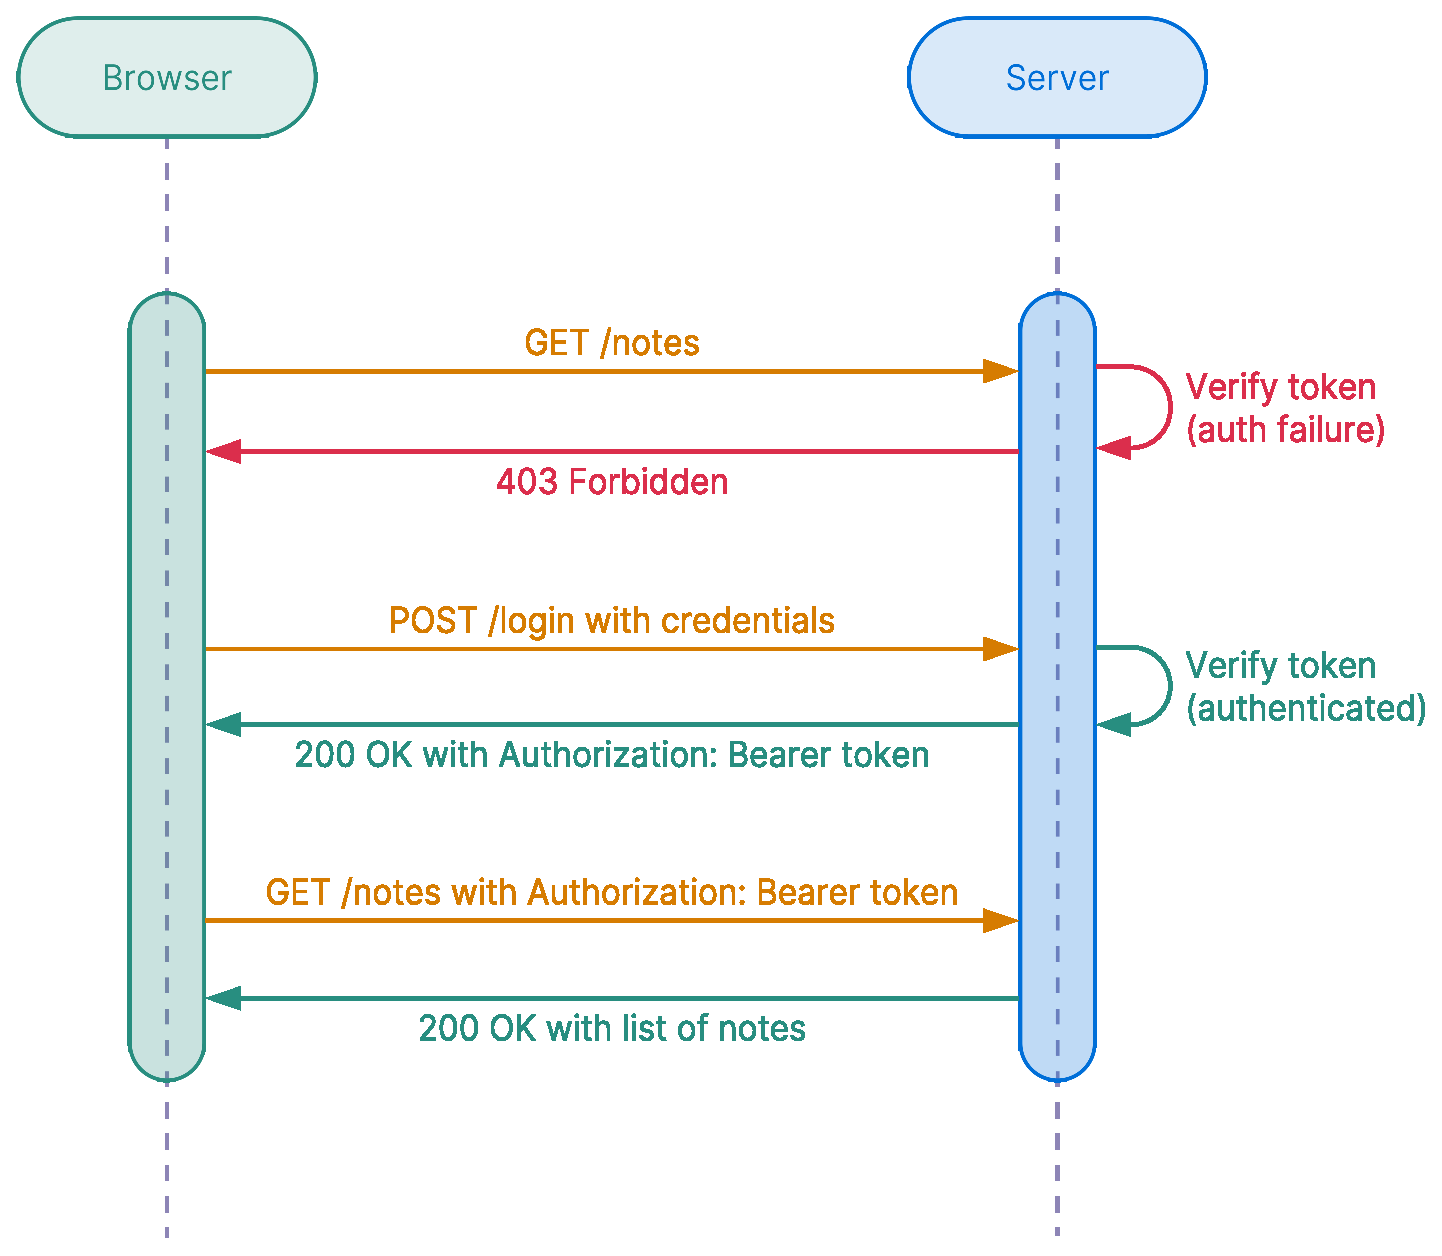
\includegraphics[scale=0.4]{images/jwt-example.eps}
        \caption{Демонстрация работы \acrshort{jwt}}
    \end{center}
\end{figure}

\textbf{\acrfull{jwt}} --- это открытый стандарт \href{https://tools.ietf.org/html/rfc7519}{(RFC 7519)}, который определяет способ для безопасной передачи информации между сторонами с помощью \acrshort{json} объектов. Эту информацию можно проверить, потому что она имеет цифровую подпись.

Вот несколько сценариев, в которых полезен \acrshort{jwt}:
\begin{itemize}
    \item \textbf{Авторизация} --- это наиболее распространенный сценарий использования \acrshort{jwt}. После того, как пользователь вошел в систему, каждый последующий запрос будет включать \acrshort{jwt}, позволяя пользователю получать доступ к маршрутам, службам и ресурсам, разрешенным с помощью этого токена.
    \item \textbf{Обмен информацией} --- \acrshort{jwt} хороший способ безопасной передачи информации между сторонами. Поскольку \acrshort{jwt} могут быть подписаны, например, с использованием пар открытого и закрытого ключей, вы можете быть уверены, что отправители являются теми, кем они себя называют. Кроме того, поскольку подпись рассчитывается с использованием \textbf{заголовка} и \textbf{полезных данных}, вы также можете убедиться, что содержимое не было изменено.
\end{itemize}

\acrshort{jwt} состоит из следующих частей:
\begin{itemize}
    \item \textbf{Заголовок} ---  содержит информацию о том, как должна вычисляться подпись. Обычно состоит из двух частей: типа токена, которым является \acrshort{jwt}, и используемого алгоритма подписи, такого как HMAC SHA256 или RSA.
    \item \textbf{Полезные данные} --- это данные, которые хранятся внутри \acrshort{jwt}. Они также называют JWT-claims (заявки). Список доступных полей для \acrshort{jwt} доступен на \href{https://en.wikipedia.org/wiki/JSON_Web_Token#Standard_fields}{Wiki}.
    \item \textbf{Подпись} --- используется для проверки того, что сообщение не было изменено в процессе. В компактной форме \acrshort{jwt} является сторой, которая состоит из трех частей, разделенных точками. Псевдокод вычисления подписи:
    \begin{noerr}
    \begin{minted}{js}
SECRET_KEY = 'some string';
unsignedToken = encodeBase64Url(header) + '.' + encodeBase64Url(payload)
signature = SHA256(unsignedToken, SECRET_KEY);

// собираем всё вместе
jwt = encodeBase64Url(header) + '.' + encodeBase64Url(payload) + '.' + encodeBase64Url(signature);
    \end{minted}
    \end{noerr}
\end{itemize}



\clearpage